\documentclass[12pt,a4paper]{article}
\usepackage{nopageno} % supress page number
\usepackage{amsmath} % displayed equations
\usepackage{amssymb} % math symbols
\usepackage[margin=0.5in]{geometry} % custom margins
\usepackage{graphicx} % figures
\usepackage{hyperref} % links in references
\usepackage{listings} % code blocks
\usepackage{color} % colored code blocks
\usepackage{caption} % custom captions
\usepackage{float} % place figures as float
\graphicspath{{./Images/}} % set path to images

% When writing indented paragraphs:
% \usepackage{indentfirst}

% Coloring of code blocks:
% Source: stackoverflow.com/a/3175141
\definecolor{dkgreen}{rgb}{0,0.6,0}
\definecolor{gray}{rgb}{0.5,0.5,0.5}
\definecolor{mauve}{rgb}{0.58,0,0.82}
\lstset{frame=tb,
  language=Java,
  aboveskip=3mm,
  belowskip=3mm,
  showstringspaces=false,
  columns=flexible,
  basicstyle={\small\ttfamily},
  numbers=none,
  numberstyle=\tiny\color{gray},
  keywordstyle=\color{blue},
  commentstyle=\color{dkgreen},
  stringstyle=\color{mauve},
  breaklines=true,
  breakatwhitespace=true,
  tabsize=3
}

\begin{document}
	\begin{center}
		% Header Image in ./Images/ folder
		% Source: extracted from https://web.northeastern.edu/ipl/wp-content/uploads/2017/09/IPL-Sample-Lab-Report.pdf
		
\includegraphics{Header}
		\vfill		
		\textbf{\Large{Report for Experiment \#N\\
		Lab Name}}
		\vfill
		Name\\
		Lab Partner: Name\\
		TA: Name\\
		Date
		\vfill
	\end{center}
	
	\section*{Abstract:}
		Summarize motivation and main results.
	
	\newpage
	
	\section*{Introduction:}
		Equations:
		\[ \vec{\nabla} \cdot \vec{E} = \frac{\rho}{\varepsilon_0} \tag{1} \]
		\[ \vec{\nabla} \cdot \vec{B} = 0 \tag{2} \]
		\[ \vec{\nabla} \times \vec{E} = - \frac{\partial \vec{B}}{\partial t} \tag{3} \]
		\[ \vec{\nabla} \times \vec{B} = \mu_0 \left( \vec{J} + \varepsilon_0 \frac{\partial \vec{E}}{\partial t} \right) \tag{4} \]
	
	\section*{Investigation n:}	
		\begin{figure}[H]
			\centering
			\begin{tabular}{ccccc}
				\(\displaystyle \vec{F}_E = \frac{1}{4 \pi \varepsilon_0} \frac{qQ}{r^2} \hat{r} \) &
				$\rightarrow$ & 
				$\displaystyle \vec{E} = \frac{1}{q} \vec{F}$ & 
				$\rightarrow$ &
				\(\displaystyle \vec{E} = \frac{1}{4 \pi \varepsilon_0} \frac{Q}{r^2} \hat{r} \)\\
				$\uparrow$ & & & & $\downarrow$\\
				\(\displaystyle \vec{F}_E = - \vec{\nabla} \Delta U\) & & & &
				\(\displaystyle \Delta V = - \int_C \vec{E} \cdot d\vec{l}\)\\
				$\uparrow$ & & & & $\downarrow$\\
				\(\displaystyle \Delta U = \frac{1}{4 \pi \varepsilon_0} \frac{Qq}{r} \) &
				$\leftarrow$ & 
				$\Delta U = q \Delta V$ & 
				$\leftarrow$ &
				\(\displaystyle \Delta V = \frac{1}{4 \pi \varepsilon_0} \frac{Q}{r} \)
			\end{tabular}
			\caption{Random Table}
		\end{figure}
		\begin{figure}[H]
			% Plot Image in ./Image/ folder
			% Source: made with InkScape
			\centering
			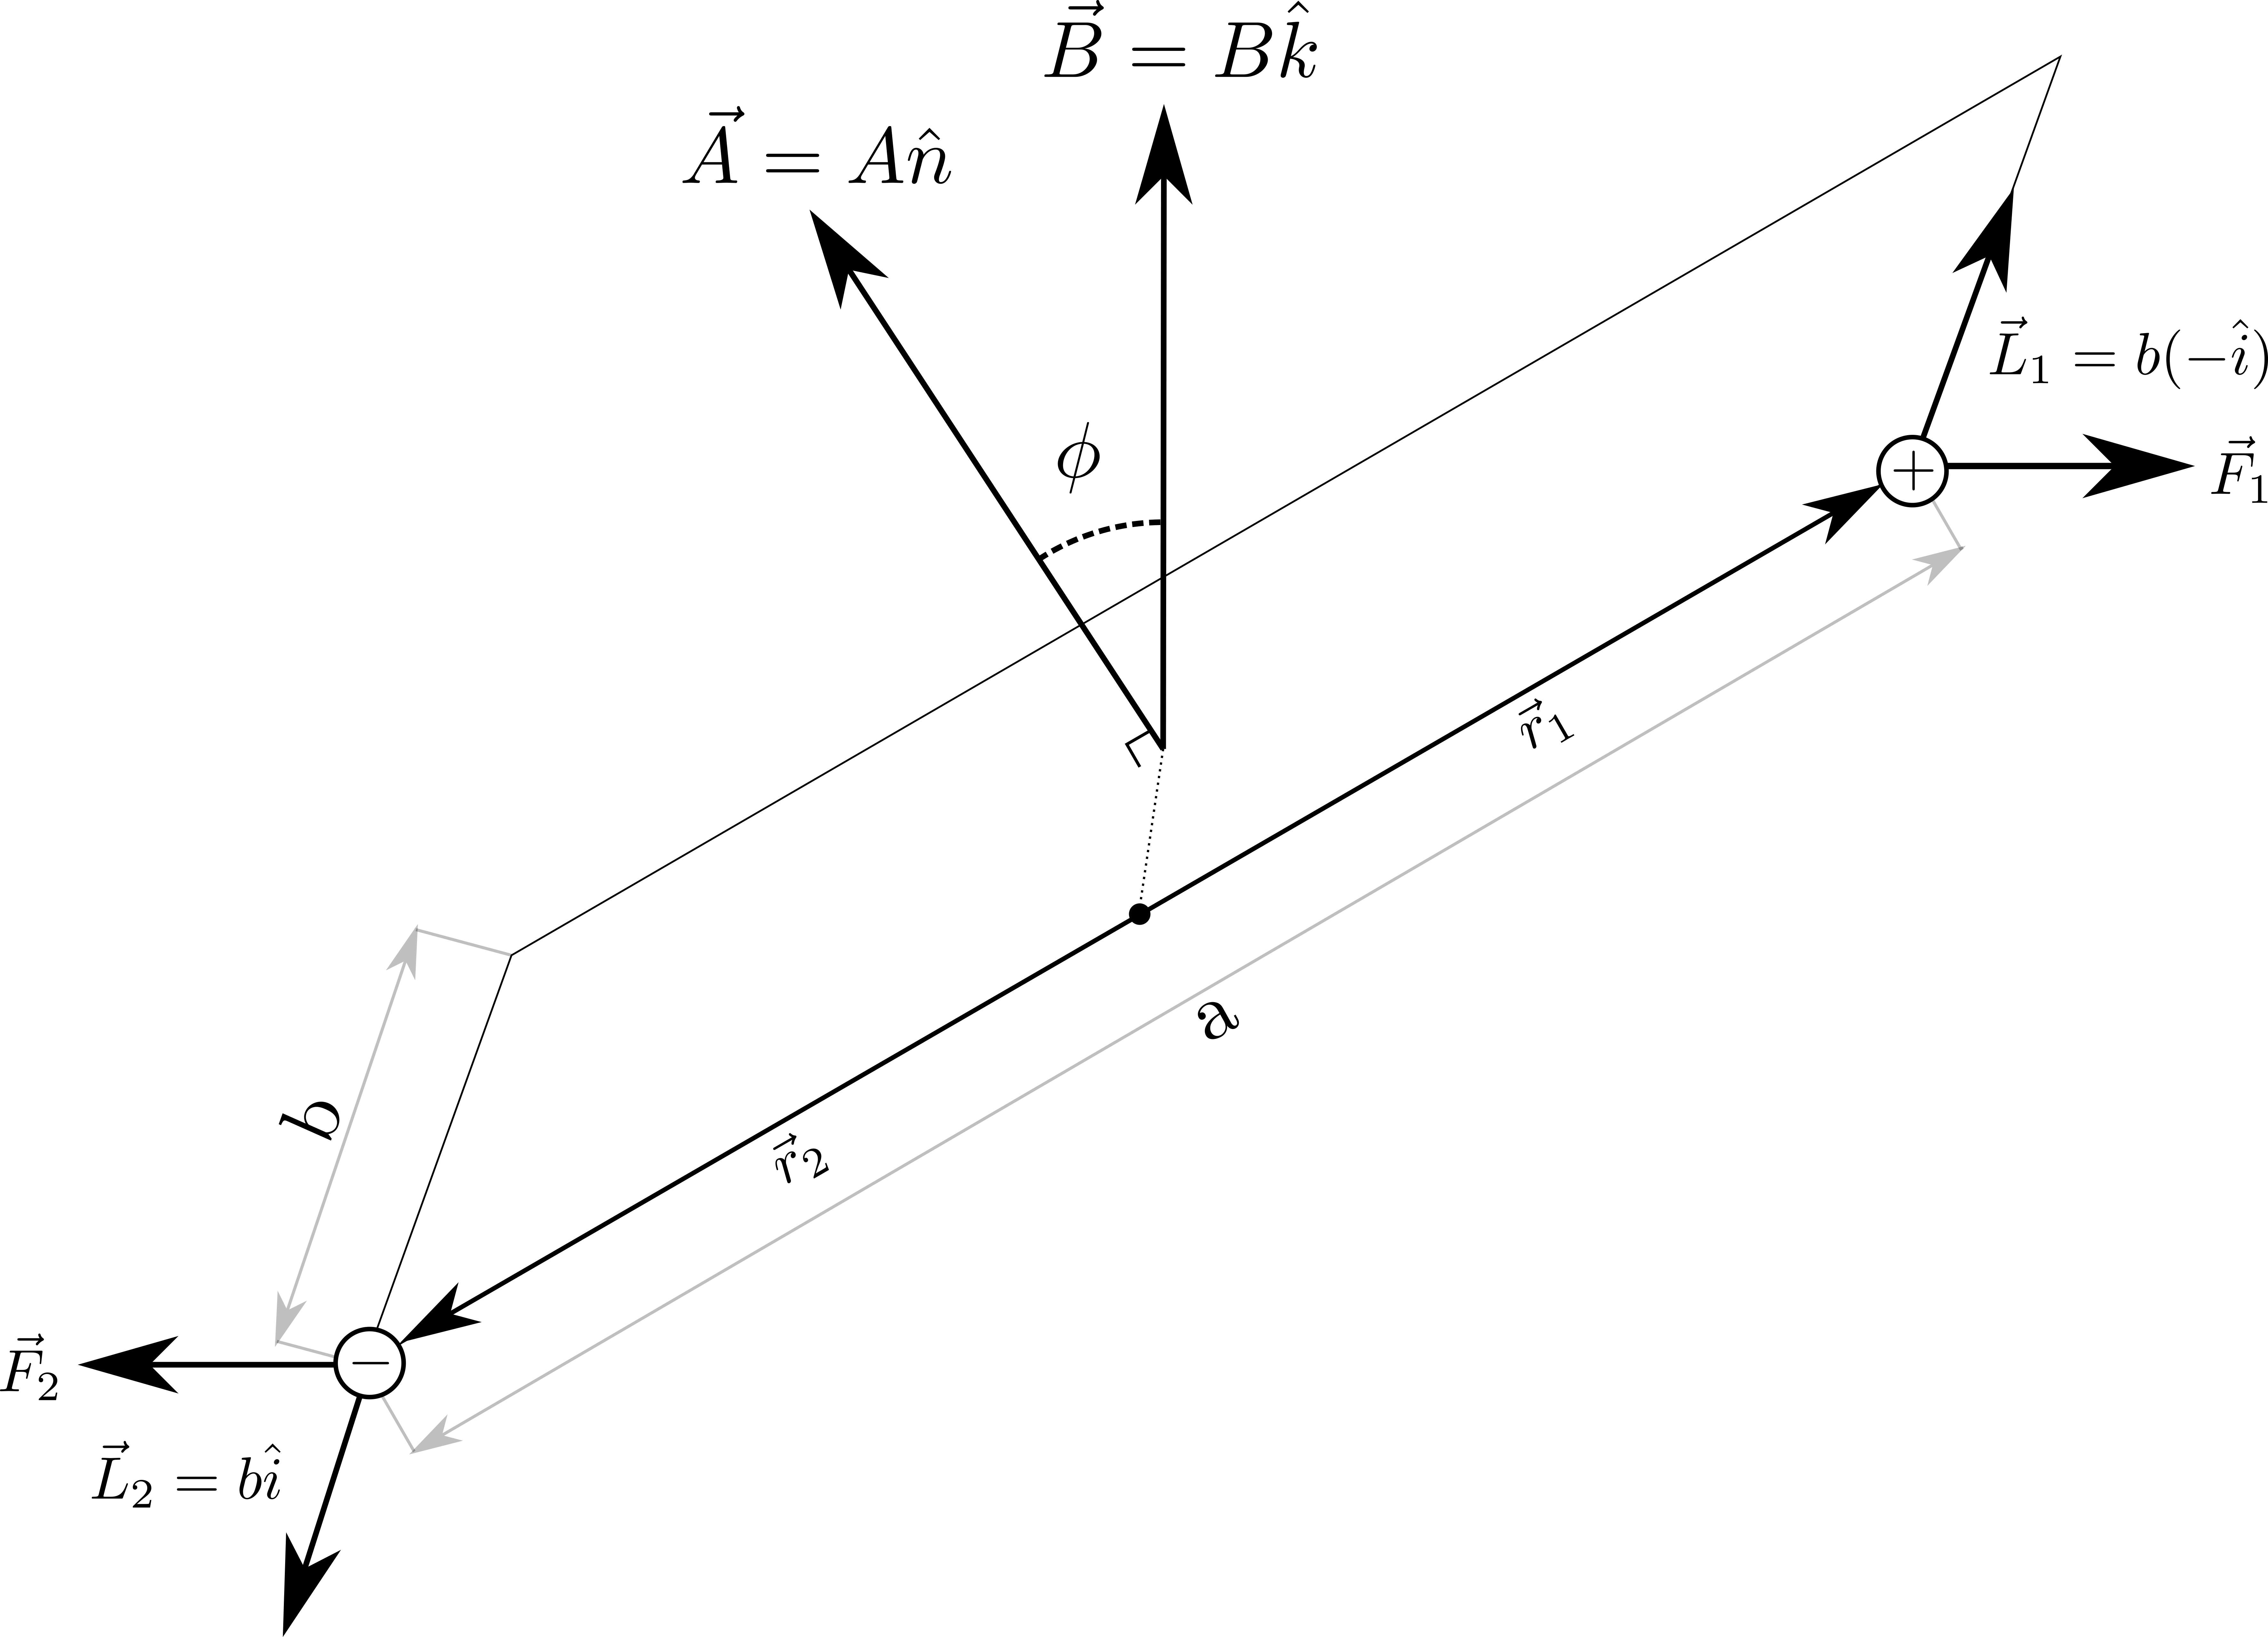
\includegraphics[width=4in]{RandFigure}\\
			\caption{Random Figure}
		\end{figure}
		\begin{figure}[H]
			\lstinputlisting[breaklines]{fibonacci.py}
			\centering
			\caption{Random Code}
		\end{figure}
		
		
	\section*{Conclusion:}
		
	\section*{Questions:}
		\begin{enumerate}
			\item Question 1
		\end{enumerate}
		
	\section*{References:}
		\begin{enumerate}
			\item \href{https://www.tablesgenerator.com/#}{Table Generator \LaTeX}, helpful if converting Excel Data
			\item \href{https://web.northeastern.edu/ipl/data-analysis/straight-line-fit/}{Northeastern IPL Straight Line Fit Calculator}
		\end{enumerate}
\end{document}